\section{Curry's Life}
Curry entered Harvard University at the age of 16 to study medicine but later switched to mathematics. After completing his undergraduate studies, he worked for two years in the electrical engineering department at the Massachusetts Institute of Technology before returning to Harvard to study physics, where he obtained a master's degree. It was during this time that Curry developed an interest in mathematical logic after taking a course on \textit{Principia Mathematica}\cite{russell25} by \textit{Whitehead}\cite{alfred-north-whitehead} and \textit{Russell}\cite{bertrand-russell}. This prompted him to pursue a doctoral degree in mathematics at Harvard.

Initially under the guidance of his mentor, George Birkoff, Curry researched differential equations. However, his fascination with mathematical logic persisted. In 1927, while at Princeton University, Curry discovered the research of Russian scholar \textit{Moses Schönfinkel}\cite{moses-schonfinkel} in the field of combinatory logic, which greatly intrigued him and solidified his commitment to the study of \textbf{Mathematical Logic}. He then traveled to Göttingen, Germany, where he collaborated with two scholars familiar with Schönfinkel's work, \textit{Heinrich Behmann}\cite{heinrich-behmann} and \textit{Paul Bernays}\cite{paul-bernays}. Under the supervision of his advisor, the renowned \textit{David Hilbert}\cite{david-hilbert}, Curry completed his doctoral thesis on combinatory logic.

Curry's career saw him teaching at Pennsylvania State College for 37 years, where he made significant contributions to the development of computer science. Following retirement, he briefly taught at the University of Amsterdam before returning to Pennsylvania State College until his passing.

\begin{figure}
    \centering
    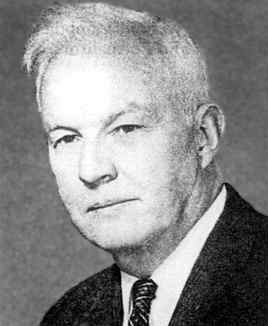
\includegraphics[width=0.3\textwidth]{figures/curry.jpg}
    \caption{Haskell Brooks Curry}
    \label{fig:curry}
\end{figure}
